\documentclass[]{tufte-book}

% ams
\usepackage{amssymb,amsmath}

\usepackage{ifxetex,ifluatex}
\usepackage{fixltx2e} % provides \textsubscript
\ifnum 0\ifxetex 1\fi\ifluatex 1\fi=0 % if pdftex
  \usepackage[T1]{fontenc}
  \usepackage[utf8]{inputenc}
\else % if luatex or xelatex
  \makeatletter
  \@ifpackageloaded{fontspec}{}{\usepackage{fontspec}}
  \makeatother
  \defaultfontfeatures{Ligatures=TeX,Scale=MatchLowercase}
  \makeatletter
  \@ifpackageloaded{soul}{
     \renewcommand\allcapsspacing[1]{{\addfontfeature{LetterSpace=15}#1}}
     \renewcommand\smallcapsspacing[1]{{\addfontfeature{LetterSpace=10}#1}}
   }{}
  \makeatother

\fi

% graphix
\usepackage{graphicx}
\setkeys{Gin}{width=\linewidth,totalheight=\textheight,keepaspectratio}

% booktabs
\usepackage{booktabs}

% url
\usepackage{url}

% hyperref
\usepackage{hyperref}

% units.
\usepackage{units}


\setcounter{secnumdepth}{2}

% citations
\usepackage{natbib}
\bibliographystyle{apalike}

% pandoc syntax highlighting

% longtable
\usepackage{longtable,booktabs}

% multiplecol
\usepackage{multicol}

% strikeout
\usepackage[normalem]{ulem}

% morefloats
\usepackage{morefloats}


% tightlist macro required by pandoc >= 1.14
\providecommand{\tightlist}{%
  \setlength{\itemsep}{0pt}\setlength{\parskip}{0pt}}

% title / author / date
\title{Improving the Reproducibility of Experimental Data Recording and Pre-Processing}
\author{Brooke Anderson, Michael Lyons, Mercedes Gonzalez-Juarrero, Marcela Henao-Tamayo, and Gregory Robertson}
\date{}

\usepackage{booktabs}
\usepackage{amsthm}
\usepackage{fontspec}
    \setmainfont{Gill Sans}
\makeatletter
\def\thm@space@setup{%
  \thm@preskip=8pt plus 2pt minus 4pt
  \thm@postskip=\thm@preskip
}
\makeatother

\begin{document}

\maketitle



{
\setcounter{tocdepth}{1}
\tableofcontents
}

\hypertarget{overview}{%
\chapter{Overview}\label{overview}}

\newthought{The recent NIH-Wide Strategic Plan} \citep{nih2016strategic}
describes an integrative view of biology and human health that includes
translational medicine, team science, and the importance of capitalizing on an
exponentially growing and increasingly complex data ecosystem \citep{nih2018data}.
Underlying this view is the need to use, share, and re-use biomedical data
generated from widely varying experimental systems and researchers. Basic
sources of biomedical data range from relatively small sets of measurements,
such as animal body weights and bacterial cell counts that may be recorded by
hand, to thousands or millions of instrument-generated data points from various
imaging, -omic, and flow cytometry experiments. In either case, there is a
generally common workflow that proceeds from measurement to data recording,
pre-processing, analysis, and interpretation. However, in practice the distinct
actions of data recording, data pre-processing, and data analysis are often
merged or combined as a single entity by the researcher using commercial or open
source spreadsheets, or as part of an often proprietary experimental measurement
system / software combination (Figure \ref{fig:workflow}), resulting in key
failure points for reproducibility at the stages of data recording and
pre-processing.

\begin{figure*}

{\centering 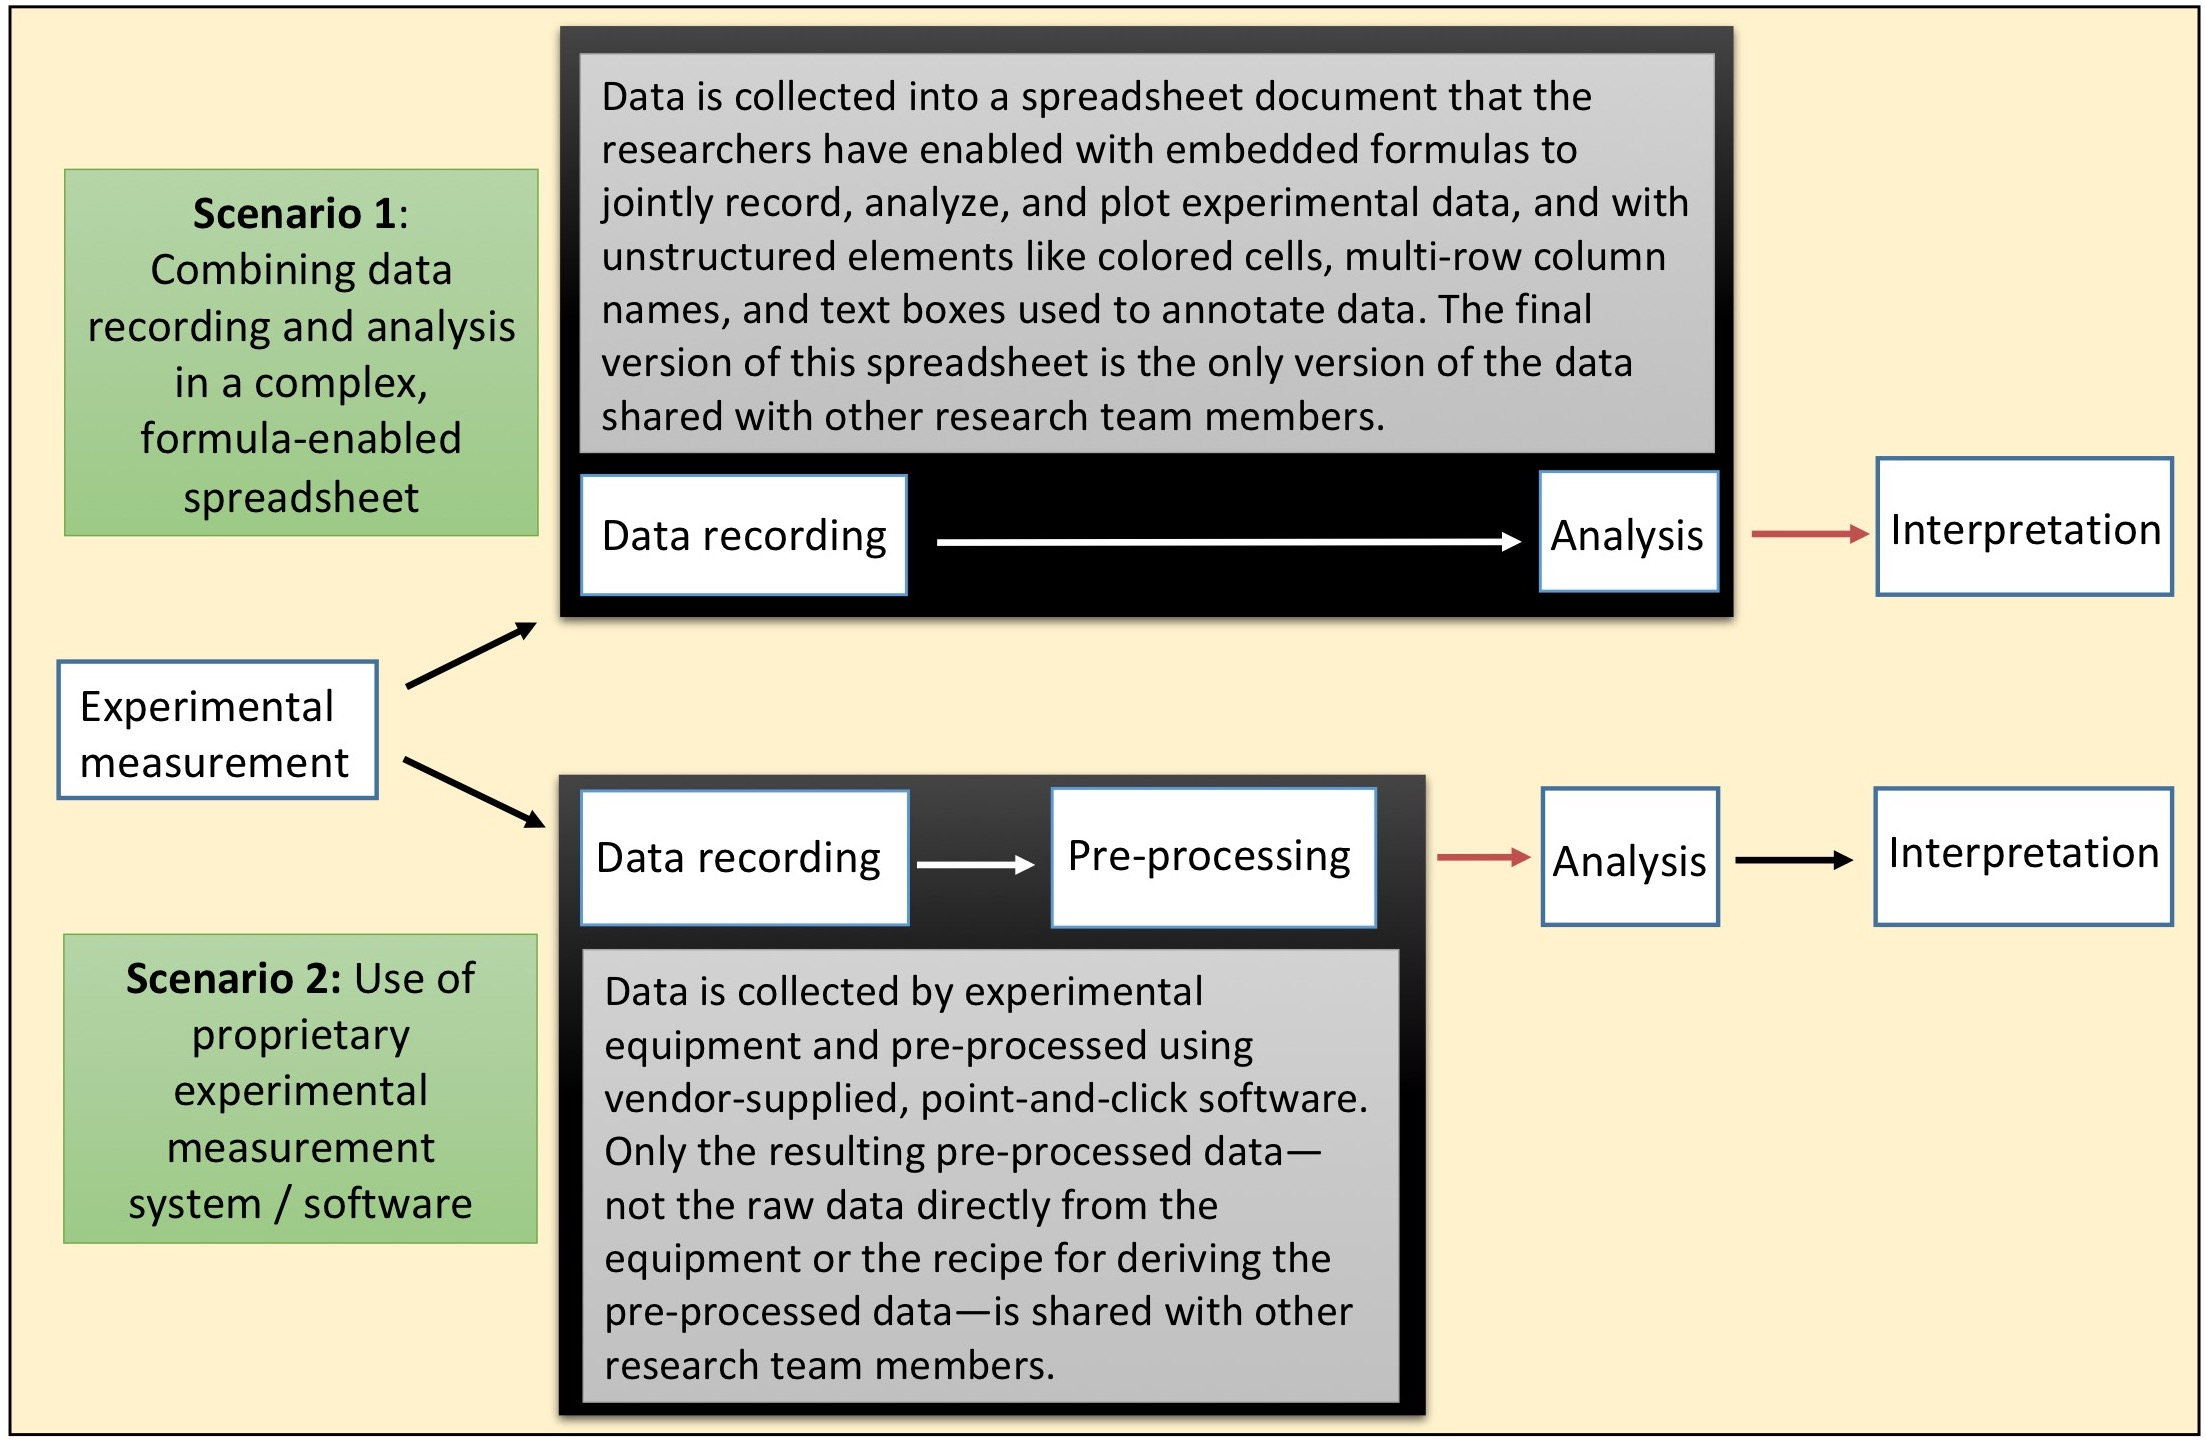
\includegraphics[width=30.64in]{figures/existing_blackboxes} 

}

\caption[Two scenarios where 'black boxes' of non-transparent, non-reproducible data handling exist in research data workflows at the stages of data recording and pre-processing]{Two scenarios where 'black boxes' of non-transparent, non-reproducible data handling exist in research data workflows at the stages of data recording and pre-processing. These create potential points of failure for reproducible research. Red arrows indicate where data is passed to other research team members, including statisticians / data analysts, often within complex or unstructured spreadsheet files.}\label{fig:workflow}
\end{figure*}

It is widely known and discussed among data scientists, mathematical modelers,
and statisticians \citep{broman2018data, krishnan2016towards} that there is
frequently a need to discard, transform, and reformat various elements of the
data shared with them by laboratory-based researchers, and that data is often
shared in an unstructured format, increasing the risks of introducing errors
through reformatting before applying more advanced computational methods.
Instead, a critical need for reproducibility is for the transparent and clear
sharing across research teams of: (1) raw data, directly from hand-recording or
directly output from experimental equipment; (2) data that has been
pre-processed as necessary (e.g., gating for flow cytometry data, feature
identification for metabolomics data), saved in a consistent, structured format,
and (3) a clear and repeatable description of how the pre-processed data was
generated from the raw data \citep{broman2018data, ellis2018share}.

To enhance data reproducibility, it is critical to create a clear separation
among data recording, data pre-processing, and data analysis---breaking up
commonly existing ``black boxes" in data handling across the research process.
Such a rigorous demarcation requires some change in the conventional
understanding and use of spreadsheets and a recognition by biomedical
researchers that recent advances in computer programming languages, especially
the R programming language, provide user-friendly and accessible tools and
concepts that can be used to extend a transparent and reproducible data workflow
to the steps of data recording and pre-processing. Among our team, we have found
that there are many common existing practices---including use of spreadsheets
with embedded formulas that concurrently record and analyze experimental data,
problematic management of project files, and reliance on proprietary,
vendor-supplied point-and-click software for data pre-processing---that can
interfere with the transparency, reproducibility, and efficiency of
laboratory-based biomedical research projects, problems that have also been
identified by others as key barriers to research reproducibility
\citep{broman2018data, bryan2018excuse, ellis2018share, marwick2018packaging}. In
these training modules, we have choosen topics that tackle barriers to
reproducibility that have straightforward, easy-to-teach solutions, but which
are still very common in biomedical laboratory-based research programs.

\hypertarget{license}{%
\section{License}\label{license}}

This book is licensed under the \href{https://creativecommons.org/licenses/by-nc-sa/4.0/}{Creative Commons
Attribution-NonCommercial-ShareAlike 4.0 International
License}, while all code in
the book is under the \href{https://opensource.org/licenses/MIT}{MIT license}.

Click on the \textbf{Next} button (or navigate using the
links at the top of the page) to continue.

\hypertarget{experimental-data-recording}{%
\chapter{Experimental Data Recording}\label{experimental-data-recording}}

\hypertarget{separating-data-recording-and-analysis}{%
\section{Separating data recording and analysis}\label{separating-data-recording-and-analysis}}

Many biomedical laboratories currently use spreadsheets---with formulas creating
underlying connections between spreadsheet cells---to jointly record, visualize,
and analyze experimental data \citep{broman2018data}. This practice impedes the
transparency and reproducibility of both data recording and data analysis. When
a research group develops and uses an evolving spreadsheet template with
embedded formulas, it leads to a data recording / analysis process that can
become extraordinarily opaque and complex. To improve the computational
reproducibility of a research project, it is critical for biomedical researchers
to learn the importance of maintaining recorded experimental data as ``read-only''
files, separating data recording from any data pre-processing or data analysis
steps \citep{broman2018data, marwick2018packaging}. Statisticians have outlined
specific methods that a laboratory-based scientist can take to ensure that data
shared in an Excel spreadsheet are shared in a reliable and reproducible way,
including avoiding macros or embedded formulas, using a separate Excel file for
each dataset, recording descriptions of variables in a separate code book rather
than in the Excel file, avoiding the use of color of the cells to encode
information, using ``NA'' to code missing values, avoiding spaces in column
headers, and avoiding splitting or merging cells \citep{ellis2018share, broman2018data}. In this module, we will describe this common practice and will
outline alternative approaches that separate the steps of data recording and
data analysis.

\textbf{Objectives.} After this module, the trainee will be able to:

\begin{itemize}
\tightlist
\item
  Explain the difference between data recording and data analysis
\item
  Understand why collecting data on spreadsheets with embedded formulas impedes
  reproducibility
\item
  List alternative approaches to improve reproducibility
\end{itemize}

\hypertarget{data-recording-versus-data-analysis}{%
\subsection{Data recording versus data analysis}\label{data-recording-versus-data-analysis}}

Many scientific laboratories use spreadsheets within their data collection
process, both to record data and to clean and analyze the data. One survey of
over 250 biomedical researchers at the University of Washington found that most
respondants used general-purpose applications like spreadsheets
\citep{anderson2007issues}, while a survey of neuroscience researchers at the
University of Newcastle similarly found that most respondents used spreadsheets
and other general-purpose software in their research \citep{altarawneh2017pilot}. A
working group on bioinformatics and data-intensive science similarly found
spreadsheets were the most common tool used across attendees
\citep{barga2011bioinformatics}.

Spreadsheets have long been an extremely popular tool, in part because they
allow people without programming experience to conduct a range of standard
computations and statistical analyses through a visual interface that is more
immediately user-friendly to non-programmers than programs with command line
interfaces. An early target for spreadsheet programs in terms of early users was
business executives, and so the programs were designed to be very simple and
easy to use---just one step up in complexity from crunching numbers on the back
of an envelope \citep{campbell2007number}. Spreadsheet programs in fact became so
popular within businesses that many attribute these programs with driving the
uptake of personal computers \citep{campbell2007number}.

Spreadsheets were innovative and rapidly adapted in part because they allowed
users to combine data recording and analysis---while previously, in business
settings, any complicated data analysis tasked needed to be outsourced to
mainframe computers and data processing teams, the initial spreadsheet program
(VisiCalc) allowed one person to quickly apply and test different models or
calculations to recorded data \citep{levy1984spreadsheet}. These spreadsheet programs
allowed non-programmers to engage with data, including data processing and
analysis tasks, that previously required programming expertise
\citep{levy1984spreadsheet}.

In some cases, a spreadsheet is used solely to record data, as a simple type of
database \citep{birch2018future}. However, biomedical researchers often use
spreadsheets to both record and analyze experimental data \citep{anderson2007issues}.
In this case, data processing and analysis is implemented through the use of
formulas and macros embedded within the spreadsheet. When a spreadsheet has
formulas or macros within it, the spreadsheet program creates an internal record
of how cells are connected through these formulas. For example, if the value in
a specific cell is converted from Fahrenheit to Celsius to fill a second cell,
and then that value is combined with other values in a column to calculate the
mean temperature across several observations, then the spreadsheet program has
internally saved how the later cells depend on the earlier ones. When you change
the value recorded in a cell of a spreadsheet, the spreadsheet program queries
this record and only recalculates the cells that depend on that cell. This
process allows the program to quickly ``react'' to any change in cell inputs,
immediately providing an update to all downstream calculations and analyses
\citep{levy1984spreadsheet}. Starting from the spreadsheet program Lotus 1-2-3,
spreadsheet programs also included \emph{macros}, ``a single computer instruction that
stands for a sequence of operations'' \citep{creeth1985microcomputer}.

Spreadsheets have become so popular in part because so many people know how to
use them, at least in basic ways, and so many people have the software on their
computers that files can be shared with the virtual guarantee that everyone will
be able to open the file on their own computer \citep{hermans2016spreadsheets}.
Spreadsheets uses the visual metaphore of a traditional gridded ledger sheet
\citep{levy1984spreadsheet}, providing an interface that is easy for users to
immediately understand and create a mental map of \citep{birch2018future, barga2011bioinformatics}. This visually clear interface also means that
spreadsheets can be printed or incorporated into other documents (Word files,
PowerPoint presentations) ``as-is'', as a workable and understandable table of
data values. In fact, some of the most popular plug-in software packages for the
early spreadsheet program Lotus 1-2-3 were programs for printing and publishing
spreadsheets \citep{campbell2007number}. This ``What You See Is What You Get''
interface was a huge advance from previous methods of data analysis for the
first spreadsheet program, VisiCalc, providing a ``window to the data'' that was
accessible to business executives and others without programming expertise
\citep{creeth1985microcomputer}. Several surveys of researchers have found that
spreadsheets were popular because of their simplicity and ease-of-use
\citep{anderson2007issues, altarawneh2017pilot, barga2011bioinformatics}. By
contrast, databases and scritped programming lanugages can be perceived as
requiring a cognitive load and lengthly training that is not worth the
investment when an easier tool is available \citep{hermans2016spreadsheets, anderson2007issues, myneni2010organization, barga2011bioinformatics, topaloglou2004biological}.

\hypertarget{hazards-of-combining-recording-and-analysis}{%
\subsection{Hazards of combining recording and analysis}\label{hazards-of-combining-recording-and-analysis}}

\textbf{Raw data often lost.}

One of the key tenets of ensuring that research is computationally reproducible
is to always keep a copy of all raw data, as well as the steps taken to get from
the raw data to a cleaned version of the data through to the results of data
analysis. However, maintaining a easily accessible copy of all original raw data
for a project is a common problem among biomedical researchers
\citep{goodman2014ten}, especially as team members move on from a laboratory group
\citep{myneni2010organization}.

The use of spreadsheets to jointly record and analyze data can contribute to
this problem. Spreadsheets allow for the immediate and embedded processing of
data. As a result, it may become very difficult to pull out the raw data
originally recorded in a spreadsheet. At the least, the combination of raw and
processed data in a spreadsheet makes it hard to identify which data points
within a spreadsheet make up the raw data and which are the result of processing
that raw data. One study of operational spreadsheets noted that:

\begin{quote}
``The data used in most spreadsheets is undocumented and there is no practical
way to check it. Even the original developer would have difficulty checking the
data.'' \citep{powell2009errors}
\end{quote}

Further, data in a spreadsheet is typically not saved as ``read-only'', so it is
possible for it to be accidentally overwritten. In situations where spreadsheets
are shared among multiple users, without ``read-only'' protection, original cell
values can easily be accidentally written over, and it may not be clear who last
changed a value, when it was changed, or why \citep{altarawneh2017pilot}.

Finally, many spreadsheets use a proprietary format. In the development of
spreadsheet programs, this use of proprietary, binary file formats helped a
software program keep users, increasing barriers for a user to switch to a new
program (since it wouldn't be able to read their old files)
\citep{campbell2007number}. However, this file format may be hard to open in the
future, as software changes and evolves \citep{michener2015ten}; by comparison, plain
text files should be widely accessible through general purpose tools regardless
of changes to proprietary software like Microsoft Excel.

\textbf{Opacity of analysis steps and potential for errors.}

Previous studies have found that errors are very common within spreadsheets
\citep{hermans2016spreadsheets}. For example, one study of 50 operational
spreadsheets found that about 90\% contained at least one error
\citep{powell2009errors}. In part, it is easier to make errors in spreadsheets and
harder to catch errors in later work with a spreadsheet because the formulas and
connections between cells aren't visible when you look at the
spreadsheet---they're behind the scenes \citep{birch2018future}. This makes it very
hard to get a clear and complete view of the pipeline of analytic steps in data
processing and analysis within a spreadsheet, as well as to discern how cells
are connected within and across sheets of the spreadsheet. As one early article on
the history of spreadsheet programs notes:

\begin{quote}
``People tend to forget that even the most elegantly crafted spreadsheet is a
house of cards, ready to collapse at the first erroneous assumption. The
spreadsheet that looks good but turns out to be tragically wrong is becoming
a familiar phenomenon.'' \citep{levy1984spreadsheet}
\end{quote}

Some characteristics of spreadsheets may heighten chances for errors. These
include high conditional complexity (i.e., lots of branching of data flow
through if / else structures), formulas that depend on a large number of cells
or that incorporate many functions \citep{hermans2016spreadsheets}. Following the
logical chain of spreadsheet formulas can be particularly difficult when several
calculations are chained in a row \citep{hermans2015enron}. Very long chains of
dependent formulas across spreadsheet cells may in some case requiring sketching
out by hand the flow of information through the spreadsheet to understand what's
going on \citep{nardi1990spreadsheet}. The use of macros can also make it
particularly hard to figure out the steps of an analysis and to diagnose and fix
any bugs in those steps \citep{nash2006spreadsheets, creeth1985microcomputer}. One
study of spreadsheets in use in real life applications noted that, ``Many
spreadsheets are so chaotically designed that auditing (especially of a few
formulas) is extremely difficult or impossible.'' \citep{powell2009errors}

In some cases, formula dependences might span across different sheets of a
spreadsheet file. For the example given above of a spreadsheet that converts
temperature from one unit to another and then averages across observations, for
example, the original temperature might be recorded in one sheet while the
converted temperature value is calculated and shown in a second sheet. These
cross-sheet dependencies can make the analysis steps even more opaque
\citep{hermans2016spreadsheets}, as a change in the cell value of one sheet might not
be immediately visible as a change in another cell on that sheet (the same is
true for spreadsheets so large that upstream and downstream cells are not
concurrently visible on screen). Other common sources of errors included
incorrect references to cells inside formulas and incorrect use of formulas
\citep{powell2009errors} or errors introduced through the common practice of copying
and pasting when developing spreadsheets \citep{hermans2016spreadsheets}.

To keep analysis steps clear, whether in scripted code or in spreadsheets or
pen-and-paper calculations, it is important to document what is being done at
each step and why \citep{goodman2014ten}. Scripted languages allow for code comments,
which are written directly into the script but not evaluated by the computer,
and so can be used to document steps within the code without changing the
operation of the code. Further, the program file itself often presents a linear,
step-by-step view of the pipeline, stored separated from the data itself
\citep{creeth1985microcomputer}. Calculations done with pen-and-paper (e.g., in a
laboratory notebook) can be annotated with text to document the steps. However,
there is evidence that spreadsheets are often poorly documented, or documented
in ways that are hard to keep track of. Before spreadsheets,

\begin{quote}
``The formulas appeared in one place and the results in another. You could see
what you were getting. That cannot be said of electronic spreadsheets, which
don't display the formulas that govern their calculations. As Mitch Kapor
explained, with electronic spreadsheets, `You can just randomly make formulas,
all of which depend on each other. And when you look at the final results, you
have no way of knowing what the rules are, unless someone tells you.'\,''
\citep{levy1984spreadsheet}
\end{quote}

Within spreadsheets, the logic and methods behind the pipeline of data
processing and analysis is often not documented, or only documented with cell
comments (hard to see as a whole) or in emails, not the spreadsheet file.
One study that investigated a large collection of spreadsheets found that most
do not include documentation explaining the logic or implementation of data
processing and analysis implemented within the spreadsheet
\citep{hermans2016spreadsheets}. A survey of neuroscience researchers at a UK
institute found that about a third of respondents included no documentation
for spreadsheets used in their research laboratories \citep{altarawneh2017pilot}.

When spreadsheet pipelines are documented, it is often through methods that are
hard to find and interpret later. One study of scientific researchers found
that, when research spreadsheets were documented, it was often through ``cell
comments'' added to specific cells in the spreadsheet, which can be hard to
interpret inclusively to understand the flow and logic of a spreadsheet as a
whole \citep{altarawneh2017pilot}. In some cases, teams discuss and document
functionality and changes in spreadsheets through email chains, passing
different versions of the spreadsheet file as attachments of emails with
discussion of the spreadsheet in the email body. One research team investigated
over 700,000 emails from employees of Enron that were released during legal
proceedings and investigated the spreadsheets attached to these emails (over
15,000 spreadsheets) as well as discussion of the spreadsheets within the emails
themselves \citep{hermans2015enron}. They found that the logic and methods of
calculations within the spreadsheets were often documented within the bodies of
emails that team members used to share and discuss spreadsheets. This means
that, if someone needs to figure out why a step was taken or identify when an
error was introduced into a spreadsheet, they may need to dig through the chain
of old emails documenting that spreadsheet, rather than being able to find the
relevant documentation within the spreadsheet's own file.

Often spreadsheets are designed, and their structure determined, by one person,
and this is often done in an \emph{ad hoc} fashion, rather than designing the
spreadsheet to follow a common structure for the research field or for the
laboratory group \citep{anderson2007issues}. Often, data processing and analysis
pipelines for spreadsheets are not carefully designed; instead, it's more
typically for spreadsheet user to start by directly entering data and formulas
without a clear overall plan \citep{altarawneh2017pilot}. Often, the person who
created the spreadsheet is the only person who fully knows how it works
\citep{myneni2010organization}, particularly if the spreadsheet includes complex
macros or a complicated structure in the analysis pipeline
\citep{creeth1985microcomputer}.

This practice creates a heavy dependence on the person who created that
spreadsheet anytime the data or results in that spreadsheet need to be
interpreted. This is particularly problematic in projects where the spreadsheet
will be shared for collaboration or adapted to be used in a future project, as
is often done in scientific research groups. One survey of neuroscience
researchers at a UK institute, for example, found that ``on average, 2--5
researchers share the same spreadsheet''. \citep{altarawneh2017pilot} In this case, it
can be hard to ``onboard'' new people to use the file, and much of the work and
knowledge about the spreadsheet can be lost when that person moves on from the
business or laboratory group \citep{creeth1985microcomputer, myneni2010organization}. If you share a spreadsheet with numerous and complex
macros and formulas included to clean and analyze the data, it can take an
extensive amount of time, and in some cases may be impossible, for the
researcher you share it with to decipher what is being done to get from the
original data input in some cells to the final results shown in others and in
graphs. Further, if others can't figure out the steps being done through macros
and formulas in a spreadsheet, they will not be able to check it for problems in
the logic of the overall analysis pipeline or for errors in the specific
formulas used within that pipeline. They also will struggle to extend and adapt
the spreadsheet to be used for other projects. These problems come up not only
when sharing with a collaborator, but also when reviewing spreadsheets that you
have previously created and used (as many have noted, your most frequent
collaborator will likely be ``future you''). In fact, one survey of biomedical
researchers at the University of Washington noted that,

\begin{quote}
``The profusion of individually created spreadsheets containing overlapping and
inconsistently updated data created a great deal of confusion within some labs.
There was little consideration to future data exchange of submission
requirements at the time of publication.'' \citep{anderson2007issues}
\end{quote}

There are methods that have been brought from more traditional programming work
into spreadsheet programming to try to help limit errors, including spreadsheet
assertions to enable testing of spreadsheets \citep{hermans2016spreadsheets}.
However, these are often not implemented, in part perhaps because many
spreadsheet users see themselves as ``end-users'', creating spreadsheets for their
own personal use rather than as something robust to future use by others, and so
don't seek out strategies adopted by ``programmers'' when creating stable tools
for others to use \citep{hermans2016spreadsheets}. In practice, though, often a
spreadsheet is used much longer, and by more people, than originally intended.
Often, the spreadsheet in this case was not designed for robust, long-term use.
From early in the history of spreadsheet programs, users have shared spreadsheet
files with interesting functionality with other users \citep{levy1984spreadsheet},
and the lifespan of a spreadsheet can be much longer than originally
intended---a spreadsheet created by one user for their own personal use can end
up being used and modified by that person or others for years
\citep{hermans2016spreadsheets}.

\textbf{Subpar software for analysis.}

While spreadsheets serve as a widely-used tool for data recording and analysis,
in many cases spreadsheets programs are poorly suited to clean and analyze
scientific data compared to other programs. As tools and interfaces continue to
develop that make other software more user-friendly to those new to programming,
scientists may want to reevaluate the costs and benefits, in terms of both time
required for training and aptness of tools, for spreadsheet programs compared to
using scripted programming languages like R and Python.

Several problems have been identified with spreadsheet programs in the context of
recording and, especially, analyzing scientific data. First, some statistical
methods may be inferior to those available in other statistical programming language.
Since the most popular spreadsheet program (Excel) is closed source, it is hard to
identify and diagnose such problems, and there is likely less of an incentive for
problems in statistical methodology to be fixed (rather than using development time
and funds to increase easier-to-see functionality in the program). Many statistical
operations require computations that cannot be perfectly achieved with a
computer, since the computer must ultimately solve many mathematical problems using
numerical approximations rather than continuous methods (e.g., calculus). The choice of
the algorithms used for these approximations heavily influence how closely a result
approximates the true answer.

A series of papers examined the quality of statistical methods in several
statistical software programs, including Excel, starting in the 1990s
\citep{mccullough1999accuracy, mccullough1999assessing, mccullough2002accuracy, mccullough2005accuracy, mccullough2008accuracy, melard2014accuracy}. In the
earliest studies, they found some concerns across all programs considered
\citep{mccullough1999accuracy, mccullough1999assessing}. One of the biggest
concerns, however, was that there was little evidence over the years that the
identified problems in Excel were resolved, or at least improved, over time
\citep{mccullough2001does, mccullough2008accuracy}. The authors note that there may
be little incentive for checking and fixing problems with algorithms for
statistical approximation in closed source software like Excel, where sales
might depend more on the more immediately evident functionality in the software,
while problems with statistical algorithms might be less evident to potential
users \citep{mccullough2001does}.

Open source software, on the other hand, offers pathways for identifying and fixing
any problems in the software, including for statistical algorithms and methods
implemented in the software's code. Since the full source code is available, researchers
can closely inspect the algorithms being used and compare them to the latest
knowledge in statistical computing methodology. Further, if an inferior algorithm is in
use, most open source software licenses allow a user to adapt and extend the software,
for example to implement better statistical algorithms.

Second, spreadsheet programs can include automated functionality that's meant to
make something easier for most users, but that might invisibly create problems
in some cases. A critical problem, for example, has been identified when using
Excel for genomics data. When Excel encounters a cell value in a format that
seems like it could be a date (e.g., ``Mar-3-06''), it will try to convert that
cell to a ``date'' class. Many software programs save date as this special ``date''
format, where it is printed and visually appears in a format like ``3-Mar-06'' but
is saved internally by the program as a number (for Microsoft Excel, the number
of days since January 1, 1900 \citep{willekens2013chronological}). By doing this, the
software can more easily undertake calculations with dates, like calculating the
number of days between two dates or which of two dates is earlier.
Bioinformatics researchers at the National Institutes of Health found that Excel
was doing this type of automatic and irreversible date conversion for 30 gene
names, including ``MAR3'' and ``APR-4'', resulting in these gene names being lost
for further analysis \citep{zeeberg2004mistaken}. Other automatic conversion problems
caused the lost of clone identifiers with composed of digits and the letter ``E''
\citep{zeeberg2004mistaken, welsh2017escape}, which were assumed to be expressing a
number using scientific notation and so automatically and irreversibly converted
to a numeric class. Further automatic conversion problems can be caused by cells
that start with an operator (e.g., ``+ control'') or with leading zeros in a
numeric identifier (e.g., ``007'') \citep{welsh2017escape}.

Avoiding this automatic date conversion required specifying that columns with
columns susceptible to these problems, including columns of gene names, should
be retained in a ``text'' class in Excel's file import process. While this
problem was originally identified and published in 2004 \citep{zeeberg2004mistaken},
along with tips to identify and avoid the problem, a study in 2016 found that
approximately a fifth of genomics papers investigated in a large-scale review
had gene name errors resulting from Excel automatic conversion, with the rate of
errors actually increasing over time \citep{ziemann2016gene}.

Finally, spreadsheet programs can be limited as analysis needs become more
complex or large \citep{topaloglou2004biological}. For example, spreadsheets can be
problematic when integrating or merging large, separate datasets
\citep{birch2018future}. This can create barriers, for example, in biological studies
seeking to integrate measurements from different instruments (e.g., flow
cytometry data with RNA-sequencing data). Further, while datasets continue to
expand in their capacity for data, for very large datasets they continue to face
limits that may be reached in practical applications \citep{birch2018future}, and
their efficiency of running data processing and analysis pipelines across large
datasets can be slow compared to code implemented with other programming
languages.

\textbf{Difficulty collaborating with statisticians.}

Modern biomedical researchers requires large teams, with statisticians and
bioinformaticians often forming a critical part of the team to enable
sophisticated processing and analysis of experimental data. However, the process
of combining data recording and analysis of experimental data, especially
through the use of spreadsheet programs, can create barriers in working across
disciplines. One group defined these issues as ``data friction'' and ``science
friction''---the extra steps and work required at each interface where data
passes, for example, from a machine to analysis or from a collaborator in one
discipline to one in a separate discipline \citep{edwards2011science}.
From a survey of scientific labs, for example, one respondent said:

\begin{quote}
``I can give data that I think are appropriate to answer a question to a
biostatistician, but when they look at it, they see it from a different point of
view. And that spreadsheet does not really encapsulate where it came from very
well, how was it generated, was it random, how was this data collected. You
would run a series of queries that you think are pertinent to what this
biostatistician would want to know. They become a part of the exploration and
not just a receiver of whatever I decided to put in my spreadsheet on that day.
What I get back is almost never fully documented in any way that I can really
understand and add more to the process.'' \citep{myneni2010organization}
\end{quote}

When collaborating with statisticians or bioinformaticians, one of the key
sources of this ``data friction'' can result from the use of spreadsheets to
jointly record and analyze experiemental data. First, spreadsheets are easy to
print or copy into another format (e.g., PowerPoint presentation, Word
document), and so researchers often design spreadsheets to be immediately
visually appealing to viewers. For example, a spreadsheet might be designed to
include hierarchically organized headers (e.g., heading and subheading, some
within a cell merged across several columns), or to show the result of a
calculation at the bottom of a column of observations (e.g., ``Total'' in the last
cell of the column) \citep{teixeira2016emergence}. Multiple separate small tables
might be included in the same sheet, with empty cells used for visual
separation, or use a ``horizontal single entry'' design , where the headers are in
the leftmost column rather than the top row \citep{teixeira2016emergence}.

These spreadsheet design choices make it much more difficult for the contents of
the spreadsheet to be read into other statistical programs. These types of data
require several extra steps in coding, in some cases fairly complex coding, with
regular expressions or logical rules needed to parse out the data and convert it
to the needed shape, before the statistical work can be done for the dataset.
This is a poor use of time for a collaborating statistician, especially if it
can be avoided through the design of the data recording template. Further, it
introduces many more chances for errors in cleaning the data.

Further, information embedded in formulas, macros, and extra formatting like
color or text boxes is lost when the spreadsheet file is input into other
programs. Spreadsheets allow users to use highlighting to represent information
(e.g., measurements for control animals shown in red, those for experiment
animals in blue) and to include information or documentation in text boxes. For
example, one survey study of biomedical researchers at the University of
Washington included this quote from a respondent: ``I have one spreadsheet that
has all of my chromosomes \ldots{} and then I've gone through and color coded it for
homozygosity and linkage.'' \citep{anderson2007issues} All the information encoded in
this sheet through color will be lost when the data from the spreadsheet is read
into another statistical program.

\hypertarget{approaches-to-separate-recording-and-analysis}{%
\subsection{Approaches to separate recording and analysis}\label{approaches-to-separate-recording-and-analysis}}

In the remaining modules in this section, we will present and describe techniques
that can be used to limit or remove these problems. First, in the module on
``Structure data'', we will walk through techniques to design data recording
formats so that data is saved in a consistent format across experiments within
a laboratory group, and in a way that removes ``data friction'' for collaboration
with statisticians or later use in scripted code. These techniques can be immediately
used to design a better spreadsheet to be used solely for data collection.

In later modules, we will discuss the use of R projects to coordinate data
recording and analysis steps within a directory, while using separate files for
data recording versus data processing and analysis. These more advanced formats
will enable the use of quality assurance / control measures like testing of data
entry and analysis functionality, better documentation of data analysis pipelines,
and easy use of version control to track projects and collaborate transparently and
with a recorded history.

{[}We will probably want to flesh this section out as we write later modules.{]}

\hypertarget{discussion-questions}{%
\subsection{Discussion questions}\label{discussion-questions}}

\hypertarget{principles-and-power-of-structured-data-formats}{%
\section{Principles and power of structured data formats}\label{principles-and-power-of-structured-data-formats}}

The format in which experimental data is recorded can have a large influence on
how easy and likely it is to implement reproducibility tools in later stages of
the research workflow. Recording data in a ``structured'' format brings many
benefits. In this module, we will explain what makes a dataset ``structured'' and
why this format is a powerful tool for reproducible research.

\textbf{Objectives.} After this module, the trainee will be able to:

\begin{itemize}
\tightlist
\item
  List the characteristics of a structured data format
\item
  Describe benefits for research transparency and reproducibility
\item
  Outline other benefits of using a structured format when recording data
\end{itemize}

\hypertarget{characteristics-of-a-structured-data-format}{%
\subsection{Characteristics of a structured data format}\label{characteristics-of-a-structured-data-format}}

\hypertarget{benefits-of-a-structured-data-format}{%
\subsection{Benefits of a structured data format}\label{benefits-of-a-structured-data-format}}

From a working group on bioinformatics and data-intensive science: ``Many simple
analyses are not automated because data formats are a moving target. \ldots{} The
community has been slow to share tools, partially because tools are not robust
against different input formats.'' \citep{barga2011bioinformatics}

``Determine whether there is a community-based metadata schema or standard (i.e.,
preferred sets of metadata elements) that can be adopted.'' \citep{michener2015ten}

First, you can still use spreadsheets, but reduce their use to recording data,
leaving all data cleaning and analysis to be handled with other software. To make
it easier to collaborate with statisticians and to interface with a program like
R for data cleaning and analysis, it will be easiest if you set up your data
recording to include with other statistical programs like R or Python. These
steps are described in a later section, ``\ldots{}''.

\begin{itemize}
\tightlist
\item
  Each sheet of the spreadsheet should contain data from a single
  experiment.
\item
  Never use whitespace to represent a meaningful separation in data within
  a spreadsheet. Never include multiple tables of data in the same sheet.
\item
  The first row of the spreadsheet should include a short column name for
  each column with data. All column name information should be within a single row
  (i.e., avoid subheadings). Avoid any special characters (e.g., ``\%'') in column
  names. Instead, use only letters, numbers, and underscores ("\_"), and start with a letter.
  It is especially helpful if you can avoid spaces in column names.
\item
  Missing data should be represented consistently in cells. ``NA'' is one choice. If
  you want to clarify why data is missing, it's much better to add a column (e.g., ``why\_missing'')
  where you can provide those details in text, rather than combining within a single column
  numerical observation data with textual reasons for missingness in cells with missing values.
\end{itemize}

Next, you could record data using a statistical language like R. There is an
excellent Integrated Development Environment for R called RStudio, and it creates a
much clearer interface with R compared to running R from a commond line, particularly for new users. RStudio allows you to open delimited plain text files, like csvs, using
a grid-style interface. This grid-style interface looks very similar to a
spreadsheet, but lacks the ability to include formulas or macros. Therefore, this
format enforces a separation of the recording of raw data from the cleaning and
analysis of the data.

{[}R Project templates{]}

Data cleaning and analysis can then be shifted away from the files used to
record the data and into reproducible scripts. These scripts can be clearly
documented, either through comments in the code or through open source
documentation tools like RMarkdown than interweave code and text in a way that
allows the creation of documents that are easier to read than commented code.

This documentation should explain why each step is being done. In cases where
it is not immediately evident from the code \emph{how} the step is being done, this
should be documented as well. Any assumptions being used should be clarified in
the documentation.

\hypertarget{applied-exercise}{%
\subsection{Applied exercise}\label{applied-exercise}}

\hypertarget{the-tidy-data-format}{%
\section{The `tidy' data format}\label{the-tidy-data-format}}

The ``tidy'' data format is an implementation of a structured data format popular
among statisticians and data scientists. By consistently using this data format,
researchers can combine simple, generalizable tools to perform complex tasks in
data processing, analysis, and visualization. We will explain what
characteristics determine if a dataset is ``tidy'' and how use of the ``tidy''
implementation of a structure data format can improve the ease and efficiency of
``Team Science''.

\textbf{Objectives.} After this module, the trainee will be able to:

\begin{itemize}
\tightlist
\item
  List characteristics defining the ``tidy'' structured data format
\item
  Explain the difference between the a structured data format (general concept)
  and the `tidy' data format (one popular implementation)
\end{itemize}

\hypertarget{the-tidy-data-format-1}{%
\subsection{The ``tidy'' data format}\label{the-tidy-data-format-1}}

\hypertarget{the-tidy-data-format-as-a-structured-data-format}{%
\subsection{The ``tidy'' data format as a structured data format}\label{the-tidy-data-format-as-a-structured-data-format}}

\hypertarget{practice-quiz}{%
\subsection{Practice quiz}\label{practice-quiz}}

\hypertarget{designing-templates-for-tidy-data-collection}{%
\section{Designing templates for ``tidy'' data collection}\label{designing-templates-for-tidy-data-collection}}

This module will move from the principles of the ``tidy'' data format to the
practical details of designing a ``tidy'' data format to use when collecting
experimental data. We will describe common issues that prevent biomedical
research datasets from being ``tidy'' and show how these issues can be avoided. We
will also provide rubrics and a checklist to help determine if a data collection
template complies with a ``tidy'' format.

\textbf{Objectives.} After this module, the trainee will be able to:

\begin{itemize}
\tightlist
\item
  Identify characteristics that keep a dataset from being `tidy'
\item
  Convert data from an ``untidy'' to a ``tidy'' format
\end{itemize}

\hypertarget{subsection-1}{%
\subsection{Subsection 1}\label{subsection-1}}

``Or maybe your goal is that your data is \emph{usable} in a wide range of
applications? If so, consider adopting standard formats and metadata
standards early on. At the very least, keep track of versions of data
and code, with associated dates.'' \citep{goodman2014ten}

``Standards for data include, for example, data formats, data exchange
protocols, and meta-data controlled vocabularies.'' \citep{barga2011bioinformatics}

\hypertarget{applied-exercise-1}{%
\subsection{Applied exercise}\label{applied-exercise-1}}

\hypertarget{example-creating-a-template-for-tidy-data-collection}{%
\section{Example: Creating a template for ``tidy'' data collection}\label{example-creating-a-template-for-tidy-data-collection}}

We will walk through an example of creating a template to collect data in a
``tidy'' format for a laboratory-based research project, based on a research
project on drug efficacy in murine tuberculosis models. We will show the initial
``untidy'' format for data recording and show how we converted it to a ``tidy''
format. Finally, we will show how the data can then easily be analyzed and
visualized using reproducible tools.

\textbf{Objectives.} After this module, the trainee will be able to:

\begin{itemize}
\tightlist
\item
  Understand how the principles of ``tidy'' data can be applied for a real, complex research project;
\item
  List advantages of the ``tidy'' data format for the example project
\end{itemize}

\hypertarget{subsection-1-1}{%
\subsection{Subsection 1}\label{subsection-1-1}}

\hypertarget{subsection-2}{%
\subsection{Subsection 2}\label{subsection-2}}

\hypertarget{discussion-questions-1}{%
\subsection{Discussion questions}\label{discussion-questions-1}}

\hypertarget{power-of-using-a-single-structured-project-directory-for-storing-and-tracking-research-project-files}{%
\section{Power of using a single structured `Project' directory for storing and tracking research project files}\label{power-of-using-a-single-structured-project-directory-for-storing-and-tracking-research-project-files}}

To improve the computational reproducibility of a research project, researchers
can use a single `Project' directory to collectively store all research data,
meta-data, pre-processing code, and research products (e.g., paper drafts,
figures). We will explain how this practice improves the reproducibility and
list some of the common components and subdirectories to include in the
structure of a `Project' directory, including subdirectories for raw and
pre-processed experimental data.

\textbf{Objectives.} After this module, the trainee will be able to:

\begin{itemize}
\tightlist
\item
  Describe a `Project' directory, including common components and subdirectories
\item
  List how a single `Project' directory improves reproducibility
\end{itemize}

\hypertarget{subsection-1-2}{%
\subsection{Subsection 1}\label{subsection-1-2}}

One study surveyed over 250 biomedical researchers at the University of Washington.
They noted that, ``a common theme surrounding data management and analysis was that
may researchers preferred to utilize their own individual methods to organize data.
The varied ways of managing data were accepted as functional for most present needs.
Some researchers admitted to having no organizational methodology at all, while others
used whatever method best suited their individual needs.'' \citep{anderson2007issues}
One respondent answered, ``They're not organized in any way---they're just thrown into
files under different projects,'' while another said ``I grab them when I need them, they're
not organized in any decent way,'' and another, ``It's not even organized---a file on a central
computer of protocols that we use, common lab protocols but those are just individual
Word files within a folder so it's not searchable per se.'' \citep{anderson2007issues}

``In general, data reuse is most possible when: 1) data; 2) metadata (information
describing the data); and 3) information about the process of generating those data,
such as code, are all provided.'' \citep{goodman2014ten}

\hypertarget{subsection-2-1}{%
\subsection{Subsection 2}\label{subsection-2-1}}

\hypertarget{practice-quiz-1}{%
\subsection{Practice quiz}\label{practice-quiz-1}}

\hypertarget{creating-project-templates}{%
\section{Creating `Project' templates}\label{creating-project-templates}}

Researchers can use RStudio's `Projects' can facilitate collecting research
files in a single, structured directory, with the added benefit of easy use of
version control. Researchers can gain even more benefits by consistently
structuring all their `Project' directories. We will demonstrate how to
implement structured project directories through RStudio, as well as how RStudio
enables the creation of a `Project' for initializing consistently-structured
directories for all of a research group's projects.

\textbf{Objectives.} After this module, the trainee will be able to:

\begin{itemize}
\tightlist
\item
  Be able to create a structured \texttt{Project} directory within RStudio
\item
  Understand how RStudio can be used to create `Project' templates
\end{itemize}

\hypertarget{subsection-1-3}{%
\subsection{Subsection 1}\label{subsection-1-3}}

\hypertarget{subsection-2-2}{%
\subsection{Subsection 2}\label{subsection-2-2}}

\hypertarget{discussion-questions-2}{%
\subsection{Discussion questions}\label{discussion-questions-2}}

\hypertarget{example-creating-a-project-template}{%
\section{Example: Creating a `Project' template}\label{example-creating-a-project-template}}

We will walk through a real example, based on the experiences of one of our
Co-Is, of establishing the format for a research group's `Project' template,
creating that template using RStudio, and initializing a new research project
directory using the created template. This example will be from a
laboratory-based research group that studies the efficacy of tuberculosis drugs
in a murine model.

\textbf{Objectives.} After this module, the trainee will be able to:

\begin{itemize}
\tightlist
\item
  Create a `Project' template in RStudio to initialize consistently-formatted
  `Project' directories
\item
  Initialize a new `Project' directory using this template
\end{itemize}

\hypertarget{subsection-1-4}{%
\subsection{Subsection 1}\label{subsection-1-4}}

\hypertarget{subsection-2-3}{%
\subsection{Subsection 2}\label{subsection-2-3}}

\hypertarget{applied-exercise-2}{%
\subsection{Applied exercise}\label{applied-exercise-2}}

\hypertarget{harnessing-version-control-for-transparent-data-recording}{%
\section{Harnessing version control for transparent data recording}\label{harnessing-version-control-for-transparent-data-recording}}

As a research project progresses, a typical practice in many experimental
research groups is to save new versions of files (e.g., `draft1.doc',
`draft2.doc'), so that changes can be reverted. However, this practice leads to
an explosion of files, and it becomes hard to track which files represent the
`current' state of a project. Version control allows researchers to edit and
change research project files more cleanly, while maintaining the power to
`backtrack' to previous versions, messages included to explain changes. We will
explain what version control is and how it can be used in research projects to
improve the transparency and reproducibility of research, particularly for data
recording.

\textbf{Objectives.} After this module, the trainee will be able to:

\begin{itemize}
\tightlist
\item
  Describe version control\\
\item
  Explain how version control can be used to improve reproducibility
  for data recording
\end{itemize}

\hypertarget{subsection-1-5}{%
\subsection{Subsection 1}\label{subsection-1-5}}

``Or maybe your goal is that your data is \emph{usable} in a wide range of
applications? If so, consider adopting standard formats and metadata
standards early on. At the very least, keep track of versions of data
and code, with associated dates.'' \citep{goodman2014ten}

\textbf{Email attachments in lieu of common access files.}

\ldots{}

For example, one group of researchers investigated a large collection of emails
from Enron \citep{hermans2015enron}. They found that passing Excel files through
email attachements was a common practice, and that messages within emails
suggested that spreadsheets were stored locally, rather than in a location that
was accessible to all team members \citep{hermans2015enron}, which meant that team
members might often be working on different versions of the same spreadsheet
file. They note that ``the practice of emailing spreadsheets is known to result in
serious problems in terms of accountability and errors, as people do not have
access to the latest version of a spreadsheet, but need to be updated of changes
via email.'' \citep{hermans2015enron}

``Team members regularly pass data files back and forth by hand, by email, and by
using shared lab or project servers, websites, and databases.''
\citep{edwards2011science}

\textbf{Version control for spreadsheets}

``Recent versions of spreadsheets now incorporate a `Traack Changes' functionality
which enables highlighting of changes made by different users along with a comment
and review system. Such tools are a start toward this but more robust version control
systems are required particularly in the context of increasingly online and
collaborative method of working where large teams interact with a single document
concurrently.'' \citep{birch2018future}

\hypertarget{subsection-2-4}{%
\subsection{Subsection 2}\label{subsection-2-4}}

\hypertarget{discussion-questions-3}{%
\subsection{Discussion questions}\label{discussion-questions-3}}

\hypertarget{enhance-the-reproducibility-of-collaborative-research-with-version-control-platforms}{%
\section{Enhance the reproducibility of collaborative research with version control platforms}\label{enhance-the-reproducibility-of-collaborative-research-with-version-control-platforms}}

Once a researcher has learned to use \emph{git} on their own computer for
local version control, they can begin using version control platforms (e.g.,
\emph{GitLab}, \emph{GitHub}) to collaborate with others under version
control. We will describe how a research team can benefit from using a version
control platform to work collaboratively.

\textbf{Objectives.} After this module, the trainee will be able to:

\begin{itemize}
\tightlist
\item
  List benefits of using a version control platform to collaborate
  on research projects, particularly for reproducibility
\item
  Describe the difference between version control (e.g., \emph{git}) and
  a version control platform (e.g., \emph{GitLab})
\end{itemize}

\hypertarget{subsection-1-6}{%
\subsection{Subsection 1}\label{subsection-1-6}}

\textbf{VC platforms as a form of back-up.}

One study surveyed neuroscience researchers at a UK institute. ``The backup `rule
of three' states that for a file to be sufficiently backed up it should be kept
in three separate locations using two different types of media with one offsite
backup. A lack of an adequate backup solution could mean permanently lost data,
effort and time. In this research, more than 82\% of the respondents seemed to be
unaware of suitable backup procedures to protect their data. Some respondents
kept a single backup of work on external hard disks. Others used the
Universities local networked servers as their means of backup.''
\citep{altarawneh2017pilot}

``A good approach is to store at least three copies in at least two
geographically distributed locations (e.g., original location such as a desktop
computer, an external hard drive, and one or more remote sites) and to adopt a
regular schedule for duplicating the data (i.e., backup).'' \citep{michener2015ten}

\hypertarget{subsection-2-5}{%
\subsection{Subsection 2}\label{subsection-2-5}}

\hypertarget{discussion-questions-4}{%
\subsection{Discussion questions}\label{discussion-questions-4}}

\hypertarget{using-git-and-gitlab-to-implement-version-control}{%
\section{Using git and GitLab to implement version control}\label{using-git-and-gitlab-to-implement-version-control}}

For many years, use of version control required use of the command line,
limiting its accessibility to researchers with limited programming experience.
However, graphical interfaces have removed this barrier, and RStudio has
particularly user-friendly tools for implementing version control. In this
module, we will show how to use \emph{git} through RStudio's user-friendly
interface and how to connect from a local computer to \emph{GitLab} through
RStudio.

\textbf{Objectives.} After this module, the trainee will be able to:

\begin{itemize}
\tightlist
\item
  Understand how to set up and use \emph{git} through RStudio's interface
\item
  Understand how to connect with \emph{GitLab} through RStudio to collaborate on\\
  research projects while maintaining version control
\end{itemize}

\hypertarget{subsection-1-7}{%
\subsection{Subsection 1}\label{subsection-1-7}}

\hypertarget{subsection-2-6}{%
\subsection{Subsection 2}\label{subsection-2-6}}

\hypertarget{applied-exercise-3}{%
\subsection{Applied exercise}\label{applied-exercise-3}}

\hypertarget{experimental-data-preprocessing}{%
\chapter{Experimental Data Preprocessing}\label{experimental-data-preprocessing}}

\hypertarget{principles-and-benefits-of-scripted-pre-processing-of-experimental-data}{%
\section{Principles and benefits of scripted pre-processing of experimental data}\label{principles-and-benefits-of-scripted-pre-processing-of-experimental-data}}

The experimental data collected for biomedical research often requires
pre-processing before it can be analyzed (e.g., gating of flow cytometry data,
feature finding / quantification for mass spectrometry data). Use of
point-and-click software can limit the transparency and reproducibility of this
analysis stage and is time-consuming for repeated tasks. We will explain how
scripted pre-processing, especially using open source software, can improve
transparency and reproducibility.

\textbf{Objectives.} After this module, the trainee will be able to:

\begin{itemize}
\tightlist
\item
  Define `pre-processing' of experimental data
\item
  Describe an open source code script and explain how it can increase
  reproducibility of data pre-processing
\end{itemize}

\hypertarget{subsection-1-8}{%
\subsection{Subsection 1}\label{subsection-1-8}}

For bioinformatics, ``all too often the software is developed without
thought toward future interoperability with other software products. As a
result, the bioinformatics software landscape is currently characterized
by fragmentation and silos, in which each research group develops and uses
only the tools created within their lab.'' \citep{barga2011bioinformatics}

``The group also noted the lack of agility. Although they may be aware of
a new or better algorithm they cannot easily integrate it into their
analysis pipelines given the lack of standards across both data formats
and tools. It typically requires a complete rewrite of the code in order
to take advntge of a new technique or algorithm, requiring time and often
funding to hire developers.'' \citep{barga2011bioinformatics}

\hypertarget{subsection-2-7}{%
\subsection{Subsection 2}\label{subsection-2-7}}

\hypertarget{discussion-questions-5}{%
\subsection{Discussion questions}\label{discussion-questions-5}}

\hypertarget{introduction-to-scripted-data-pre-processing-in-r}{%
\section{Introduction to scripted data pre-processing in R}\label{introduction-to-scripted-data-pre-processing-in-r}}

We will show how to implement scripted pre-processing of experimental data
through R scripts. We will demonstrate the difference between interactive coding
and code scripts, using R for examples. We will then demonstrate how to create,
save, and run an R code script for a simple data cleaning task.

\textbf{Objectives.} After this module, the trainee will be able to:

\begin{itemize}
\tightlist
\item
  Describe what an R code script is and how it differs from interactive
  coding in R
\item
  Create and save an R script to perform a simple data pre-processing task
\item
  Run an R script
\item
  List some popular packages in R for pre-processing biomedical data
\end{itemize}

\hypertarget{subsection-1-9}{%
\subsection{Subsection 1}\label{subsection-1-9}}

\hypertarget{subsection-2-8}{%
\subsection{Subsection 2}\label{subsection-2-8}}

\hypertarget{applied-exercise-4}{%
\subsection{Applied exercise}\label{applied-exercise-4}}

\hypertarget{simplify-scripted-pre-processing-through-rs-tidyverse-tools}{%
\section{Simplify scripted pre-processing through R's `tidyverse' tools}\label{simplify-scripted-pre-processing-through-rs-tidyverse-tools}}

The R programming language now includes a collection of `tidyverse' extension
packages that enable user-friendly yet powerful work with experimental data,
including pre-processing and exploratory visualizations. The principle behind
the `tidyverse' is that a collection of simple, general tools can be joined
together to solve complex problems, as long as a consistent format is used for
the input and output of each tool (the `tidy' data format taught in other
modules). In this module, we will explain why this `tidyverse' system is so
powerful and how it can be leveraged within biomedical research, especially for
reproducibly pre-processing experimental data.

\textbf{Objectives.} After this module, the trainee will be able to:

\begin{itemize}
\tightlist
\item
  Define R's `tidyverse' system
\item
  Explain how the `tidyverse' collection of packages can be both user-friendly
  and powerful in solving many complex tasks with data
\item
  Describe the difference between base R and R's `tidyverse'.
\end{itemize}

\hypertarget{subsection-1-10}{%
\subsection{Subsection 1}\label{subsection-1-10}}

\hypertarget{subsection-2-9}{%
\subsection{Subsection 2}\label{subsection-2-9}}

\hypertarget{practice-quiz-2}{%
\subsection{Practice quiz}\label{practice-quiz-2}}

\hypertarget{complex-data-types-in-experimental-data-pre-processing}{%
\section{Complex data types in experimental data pre-processing}\label{complex-data-types-in-experimental-data-pre-processing}}

Raw data from many biomedical experiments, especially those that use
high-throughput techniques, can be very large and complex. Because of the scale
and complexity of these data, software for pre-processing the data in R often
uses complex, `untidy' data formats. While these formats are necessary for
computational efficiency, they add a critical barrier for researchers wishing to
implement reproducibility tools. In this module, we will explain why use of
complex data formats is often necessary within open source pre-processing
software and outline the hurdles created in reproducibility tool use among
laboratory-based scientists.

\textbf{Objectives.} After this module, the trainee will be able to:

\begin{itemize}
\tightlist
\item
  Explain why R software for pre-processing biomedical data often stores
  data in complex, `untidy' formats
\item
  Describe how these complex data formats can create barriers to
  laboratory-based researchers seeking to use reproducibility tools for
  data pre-processing
\end{itemize}

\hypertarget{subsection-1-11}{%
\subsection{Subsection 1}\label{subsection-1-11}}

\hypertarget{subsection-2-10}{%
\subsection{Subsection 2}\label{subsection-2-10}}

\hypertarget{practice-quiz-3}{%
\subsection{Practice quiz}\label{practice-quiz-3}}

\hypertarget{complex-data-types-in-r-and-bioconductor}{%
\section{Complex data types in R and Bioconductor}\label{complex-data-types-in-r-and-bioconductor}}

Many R extension packages for pre-processing experimental data use complex
(rather than `tidy') data formats within their code, and many output data in
complex formats. Very recently, the \emph{broom} and \emph{biobroom} R
packages have been developed to extract a `tidy' dataset from a complex data
format. These tools create a clean, simple connection between the complex data
formats often used in pre-processing experimental data and the `tidy' format
required to use the `tidyverse' tools now taught in many introductory R courses.
In this module, we will describe the `list' data structure, the common backbone
for complex data structures in R and provide tips on how to explore and extract
data stored in R in this format, including through the \emph{broom} and
\emph{biobroom} packages.

\textbf{Objectives.} After this module, the trainee will be able to:

\begin{itemize}
\tightlist
\item
  Describe the structure of R's `list' data format
\item
  Take basic steps to explore and extract data stored in R's complex, list-based
  structures
\item
  Describe what the \emph{broom} and \emph{biobroom} R packages can do
\item
  Explain how converting data to a `tidy' format can improve reproducibility
\end{itemize}

\hypertarget{subsection-1-12}{%
\subsection{Subsection 1}\label{subsection-1-12}}

\hypertarget{subsection-2-11}{%
\subsection{Subsection 2}\label{subsection-2-11}}

\hypertarget{applied-exercise-5}{%
\subsection{Applied exercise}\label{applied-exercise-5}}

\hypertarget{example-converting-from-complex-to-tidy-data-formats}{%
\section{Example: Converting from complex to `tidy' data formats}\label{example-converting-from-complex-to-tidy-data-formats}}

We will provide a detailed example of a case where data pre-processing in R
results in a complex, `untidy' data format. We will walk through an example of
applying automated gating to flow cytometry data. We will demonstrate the
complex initial format of this pre-processed data and then show trainees how a
`tidy' dataset can be extracted and used for further data analysis and
visualization using the popular R `tidyverse' tools. This example will use real
experimental data from one of our Co-Is research on the immunology of
tuberculosis.

\textbf{Objectives.} After this module, the trainee will be able to:

\begin{itemize}
\tightlist
\item
  Describe how tools like \textit{biobroom} were used in this real research
  example to convert from the complex data format from pre-processing to a format
  better for further data analysis and visualization
\item
  Understand how these tools would fit in their own research pipelines
\end{itemize}

\hypertarget{subsection-1-13}{%
\subsection{Subsection 1}\label{subsection-1-13}}

\hypertarget{subsection-2-12}{%
\subsection{Subsection 2}\label{subsection-2-12}}

\hypertarget{applied-exercise-6}{%
\subsection{Applied exercise}\label{applied-exercise-6}}

\hypertarget{introduction-to-reproducible-data-pre-processing-protocols}{%
\section{Introduction to reproducible data pre-processing protocols}\label{introduction-to-reproducible-data-pre-processing-protocols}}

Reproducibility tools can be used to create reproducible data pre-processing
protocols---documents that combine code and text in a `knitted' document, which
can be re-used to ensure data pre-processing is consistent and reproducible
across research projects. In this module, we will describe how reproducible data
pre-processing protocols can improve reproducibility of pre-processing
experimental data, as well as to ensure transparency, consistency, and
reproducibility across the research projects conducted by a research team.

\textbf{Objectives.} After this module, the trainee will be able to:

\begin{itemize}
\tightlist
\item
  Define a `reproducible data pre-processing protocol'
\item
  Explain how such protocols improve reproducibility at the data pre-processing
  phase
\item
  List other benefits, including improving efficiency and consistency of data
  pre-processing
\end{itemize}

\hypertarget{subsection-1-14}{%
\subsection{Subsection 1}\label{subsection-1-14}}

\hypertarget{subsection-2-13}{%
\subsection{Subsection 2}\label{subsection-2-13}}

\hypertarget{discussion-questions-6}{%
\subsection{Discussion questions}\label{discussion-questions-6}}

\hypertarget{rmarkdown-for-creating-reproducible-data-pre-processing-protocols}{%
\section{RMarkdown for creating reproducible data pre-processing protocols}\label{rmarkdown-for-creating-reproducible-data-pre-processing-protocols}}

The R extension package RMarkdown can be used to create documents that combine
code and text in a `knitted' document, and it has become a popular tool for
improving the computational reproducibility and efficiency of the data analysis
stage of research. This tool can also be used earlier in the research process,
however, to improve reproducibility of pre-processing steps. In this module, we
will provide detailed instructions on how to use RMarkdown in RStudio to create
documents that combine code and text. We will show how an RMarkdown document
describing a data pre-processing protocol can be used to efficiently apply the
same data pre-processing steps to different sets of raw data.

\textbf{Objectives.} After this module, the trainee will be able to:

\begin{itemize}
\tightlist
\item
  Define RMarkdown and the documents it can create
\item
  Explain how RMarkdown can be used to improve the reproducibility of research
  projects at the data pre-processing phase
\item
  Create a document in RStudio using
\item
  Apply it to several different datasets with the same format
\end{itemize}

\hypertarget{subsection-1-15}{%
\subsection{Subsection 1}\label{subsection-1-15}}

\hypertarget{subsection-2-14}{%
\subsection{Subsection 2}\label{subsection-2-14}}

\hypertarget{applied-exercise-7}{%
\subsection{Applied exercise}\label{applied-exercise-7}}

\hypertarget{example-creating-a-reproducible-data-pre-processing-protocol}{%
\section{Example: Creating a reproducible data pre-processing protocol}\label{example-creating-a-reproducible-data-pre-processing-protocol}}

We will walk through an example of creating a reproducible protocol for the
automated gating of flow cytometry data for a project on the immunology of
tuberculosis lead by one of our Co-Is. This data pre-processing protocol was
created using RMarkdown and allows the efficient, transparent, and reproducible
gating of flow cytometry data for all experiments in the research group. We will
walk the trainees through how we developed the protocol initially, the final
pre-processing protocol, how we apply this protocol to new experimental data.

\textbf{Objectives.} After this module, the trainee will be able to:

\begin{itemize}
\tightlist
\item
  Explain how a reproducible data pre-processing protocol can be integrated into
  a real research project
\item
  Understand how to design and implement a data pre-processing protocol to
  replace manual or point-and-click data pre-processing tools
\end{itemize}

\hypertarget{subsection-1-16}{%
\subsection{Subsection 1}\label{subsection-1-16}}

\hypertarget{subsection-2-15}{%
\subsection{Subsection 2}\label{subsection-2-15}}

\hypertarget{practice-quiz-4}{%
\subsection{Practice quiz}\label{practice-quiz-4}}

\hypertarget{references}{%
\chapter{References}\label{references}}

\bibliography{book.bib,packages.bib}



\end{document}
